\subsubsection{Brain Networks}
\index{Hilgetag, Claus C.}

\paragraph{Research Team}
Claus C. Hilgetag (Professor), Yu Jin (Postdoc),  Stoyan Kurtev (PhD Student)\\


Research in our group focuses on central questions of systems neuroscience:
How are the complex neural networks in the brain organized structurally and functionally?  How do specialized brain regions interact in distributed brain networks in order to produce unified brain function?

We investigate these problems theoretically, through computational and multivariate
statistical analyses of complex neuroanatomic data for the primate brain, and experimentally,
by applying 'virtual lesions' (produced by transcranial magnetic stimulation, TMS) to brain
regions dealing with spatial attention in the human brain. The goal of these approaches is to determine the specificity and global structural organization of primate cortical brain regions and their multiple anatomical interconnections. We also aim to understand how the structural organization of the brain underlies its diverse, efficient and robust functions.


\paragraph{Highlights}
%
In 2006, we published a number of widely noticed research findings. First, in a joint study with Helen Barbas of Boston University, we demonstrated that the layout of nerve fiber connections among brain regions (Fig.~\ref{fig:Hilgetag_2005_fig}) underlies the characteristically folded landscape of the primate brain (Hilgetag \& Barbas 2006).  The brain landscape is shaped into hills and valleys by the combined pulling forces produced by the fibers.  Moverover, several other aspects of the shape of the brain, for example the regional thickness of the cerebral cortex, are also influenced by mechanical forces.

Second, in another computational study we demonstrated that the primate brain is not optimized for overall minimal wiring of neural connections, as had been widely assumed so far.  Instead, a mix of short and long connections supports efficient neural processing in combination with a small volume of the brain.  This work was carried out together with former graduate student Marcus Kaiser, who now holds an Academic Fellowship at Newcastle University, UK.

Third, in joint work with Jarrett Rushmore and Antoni Valero-Cabre of Boston University School of Medicine, we showed that impairements of visual attention produced by lesions in one hemisphere of the cat brain can be reversed by subsequent deactivation of a midbrain structure (the superior colliculus) in the contralateral brain hemisphere. This finding has implications for the rehabilitation of human patients after strokes or other brain damage.


% to include a figure, generate a file xxx.pdf and integrate the following lines
\begin{figure}[ht]
  \begin{center}
    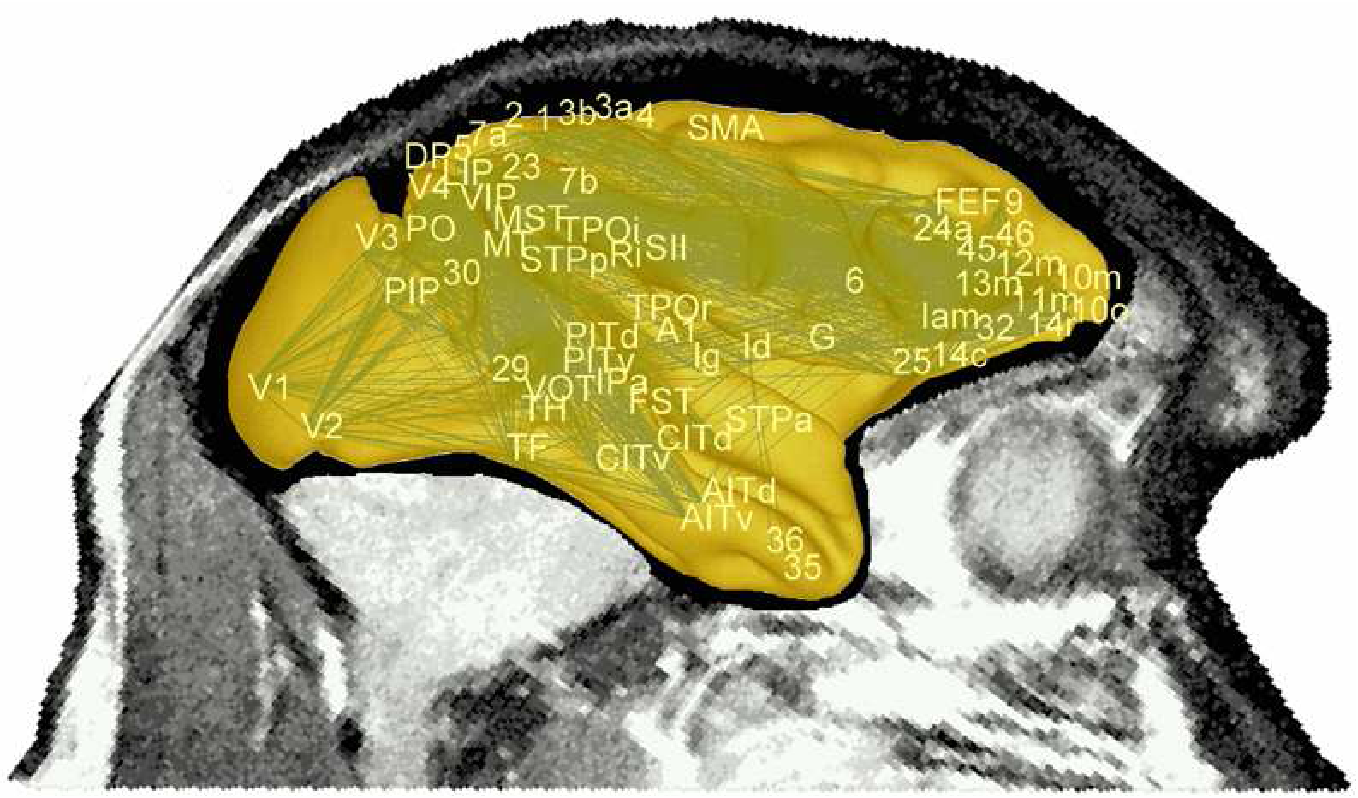
\includegraphics[width=\hsize]{Hilgetag/Hilgetag_2005_fig.pdf}
    \mycaption{The intricate network of neural projections interlinking cerebral cortical areas in the brain of the rhesus monkey.}
    \label{fig:Hilgetag_2005_fig}
  \end{center}
\end{figure}


\myparagraph{Collaborations}
%
Bremen Area Collaborations:
\begin{enumerate}
\item {\sl International University Bremen }\\Prof. A. Diederich, Prof. B. Olk\\Networks for Spatial Attention and Eye Movement in the Human
\\ Prof. G.K.H. Zupanc \\ Modeling of development of neural networks
\item {\sl Universit\"{a}t Bremen}\\Prof. M. Fahle\\Functions
of the Human Visual Cortex Explored by ``Virtual Lesions''
Brain

\end{enumerate}
National \& International Collaborations:
\begin{enumerate}
\item {\sl Boston University, Boston, USA}\\Prof. H. Barbas\\Computational
Mapping of Primate Prefrontal Cortical Architecture and Connections
\item {\sl City University London, London, UK}\\Dr. S. Grant\\Linking
Architecture and Connectivity in the Cat Extrastriate Cortex
\item {\sl Newcastle University (formerly Jacobs University), Newcastle, UK}\\Dr. M.
Kaiser\\Organization, Development and Function of Cortical Brain
Networks
\item {\sl Tel-Aviv University, Tel-Aviv, Israel}\\Prof. E. Ruppin, Dr. A.
Kaufman\\Functional Contributions in Neural Networks Derived from
Lesion Analysis
\item {\sl Boston University School of Medicine, Boston, USA}\\Dr. A. Valero-Cabre, Dr. J.
Rushmore\\Mechanisms of Intact, Impaired and Restored Spatial
Attention in the Mammalian Brain
\end{enumerate}

\paragraph{Grants}
% list the running grants in 2005, if none have been received, please delete this
% subsection.
\begin{enumerate}
\item Funded by DAAD-PPP, \emph{Computational Mapping of the
Primate Prefrontal Cortex},  (January 2005 - December 2007)
\end{enumerate}

\paragraph{Other Support Grants}
% list the running grants in 2005, if none have been received, please delete this
% subsection.
\begin{enumerate}
\item {\sl NIH (NIMH) R01}, Organization of Prefrontal Feedback Circuits
(2004-2009), Investigator (PI: H. Barbas)
\item {\sl NIH (NINDS) R01} Prefrontal Anatomic Pathways in Executive Control
 (2005-2010), Investigator (PI: H. Barbas)
 \end{enumerate}


\nocite{Hilgetag1,Hilgetag2,Hilgetag3,Hilgetag4,Hilgetag5,Hilgetag6, Hilgetag7,Hilgetag8,hilgetag9,hilgetag10}
